% !TEX root = ../algo-summary.tex
\section{Dynamic Programming}\label{sec:dynamic_programming}


\textcolor{AccentBlue}{Greedy}. 
Build up a solution incrementally, myopically optimizing some local criterion.

\medskip

\textcolor{AccentBlue}{Divide-and-conquer}. 
Break up a problem into two sub-problems of roughly equal size; 
solve each sub-problem independently; 
combine the two sub-problem solutions to form solution to original problem.

\medskip

\textcolor{AccentRed}{Dynamic programming}. 
Break up a problem into many overlapping sub-problems; 
combine solutions to small subproblems to build up solutions to larger and larger sub-problems.
\begin{itemize}
\item overlapping sub-problem = a sub-problem whose results can be reused many times
\item Hint: express your optimal solution by a recursive formula
\end{itemize}

\medskip

\textcolor{AccentBlue}{Some famous dynamic programming algorithms}:
\begin{itemize}
  \item Viterbi for Hidden Markov Models
  \item Unix diff for comparing two files
  \item Smith-Waterman for sequence alignment
  \item \nameref{alg:bellmanford} for shortest path routing in networks
  \item Cocke-Kasami-Younger for parsing context-free grammars
\end{itemize}


\bigskip


Powerful technique for solving optimization problems, which have certain well-defined clean structural properties.

\bigskip

\begin{definition}[Principle of optimality]\label{def:principle_of_optimality}
\hl[5]{For the global problem to be solved optimally, each subproblem must be solved optimally.}
\end{definition}
\indent \(\rightarrow\) this principle must hold to apply DP

\bigskip
\smallskip

The global optimal solution consists of optimal solutions to subproblems.

\medskip
Polynomial time DP:
\begin{itemize}
\item Polynomially-many distinct overlapping subproblems (polynomial in input size).
\item DP does not necessarily lead to a polynomial time algorithm
\end{itemize}
\medskip

DP selection principle: \hl{When given a set of feasible options to choose from, try them all and take the best}












\subsection{Weighted Interval Scheduling}








We denote by \(p(j)\) the largest index \(i\) with \(i < j\) and such that job \(i\) is compatible with \(j\), i.e.
\begin{equation}\label{eq:interval_scheduling_pj}
  p(j)
  :=
  \begin{cases}
    \max\{ i \mid f_i \leq s_j\} & \exists i \text{ with } f_i \leq s_j\\
    0 & \text{otherwise}
  \end{cases}
\end{equation}



\begin{algorithm}[h]
\caption{Compute \(p(j)\) values}\label{alg:compute_pj}
\begin{algorithmic}[1]
\Require Jobs \(1, \ldots, n\) sorted according to their finish time \(f_1 \leq \cdots \leq f_n\)
\State Sort all starting and finish times in a single array \(A\)
\State \(\texttt{index} \gets 0\)
\ForAll{\(e \in A\)} \Comment{go through all times (`events') in ascending order}
  \If{\(e = f_i\)}
    \State \(\texttt{index} \gets i\)
  \ElsIf{\(e = s_j\)}
    \State \(p[j] \gets \texttt{index}\)
  \EndIf
\EndFor
\end{algorithmic}
\end{algorithm}

The algorithm goes through every time slot, and it remembers the index of the last finish time.
When we encounter a starting time $s_j$, its $p$ value is the largest index $i$ such that $f_i \leq s_j$, which is exactly the value of \texttt{index} in the algorithm. 
Hence, \autoref{alg:compute_pj} is correct.

Sorting takes $O(n \log n)$ time, and it is easy to see that the for loop takes $O(n)$ time.



% \textcolor{AccentBlue}{Dynamic programming formulation.}
Assume jobs are labeled so that \(f_1 \le \cdots \le f_n\).
Let \(v_j\) be the value/weight of job \(j\), and let
\(
\operatorname{OPT}(j)
\)
denote the maximum total weight of a subset of mutually compatible jobs among \(1,\ldots,j\).
We use the convention \(\operatorname{OPT}(0) = 0\).

\textcolor{AccentBlue}{Recurrence.}
For \(j \ge 1\) we have
\[
\operatorname{OPT}(j)
=
\max\bigl\{
  v_j + \operatorname{OPT}(p(j)),\;
  \operatorname{OPT}(j-1)
\bigr\}
\]
\begin{itemize}
  \item Either the optimal solution does \emph{not} take job \(j\): then its value is \(\operatorname{OPT}(j-1)\).
  \item Or the optimal solution \emph{does} take job \(j\): then we gain \(v_j\) plus the best compatible subset among jobs \(\{1,\ldots,p(j)\}\), which has value \(\operatorname{OPT}(p(j))\).
\end{itemize}

% To reconstruct an optimal set of jobs, start from \(j = n\) and trace backwards:
% \begin{itemize}
%   \item if \(v_j + \operatorname{OPT}[p[j]] \ge \operatorname{OPT}[j-1]\) then take job \(j\) and continue with \(p(j)\);
%   \item otherwise skip job \(j\) and continue with \(j-1\).
% \end{itemize}


\begin{algorithm}[h]
\caption{Weighted Interval Scheduling}\label{alg:weighted_interval_scheduling_dp}
\begin{algorithmic}[1]
\Require jobs \(1,\ldots,n\) sorted by finish time, values \(v_j\), and precomputed \(p(j)\) as in \eqref{eq:interval_scheduling_pj}
\State \(\operatorname{OPT}[0] \gets 0\)
\For{$j = 1 \TO n$}
  \State \(\operatorname{OPT}[j] \gets \max\{\,v_j + \operatorname{OPT}[p[j]],\; \operatorname{OPT}[j-1]\,\}\)
\EndFor
\State \Return \(\operatorname{OPT}[n]\)
\end{algorithmic}
\end{algorithm}

\textcolor{AccentBlue}{Running time.}
Computing the \(\operatorname{OPT}[j]\) table takes \(O(n)\) time once the jobs are sorted and the \(p(j)\) values are known.
Together with sorting and the \(p(j)\)-computation, the total running time is \(O(n \log n)\) and the space usage is \(O(n)\).


\subsection{Segmented Least Squares}
Given \(n\) points \((x_1,y_1),\ldots,(x_n,y_n)\) in the plane (assume \(x_1 < \cdots < x_n\)),
we want to approximate them by a small number of straight-line segments.

\begin{itemize}
  \item For any \(1 \le i \le j \le n\), consider fitting a single line to the points
        \((x_i,y_i),\ldots,(x_j,y_j)\) by least squares.
  \item Let \(e(i,j)\) be the sum of squared vertical errors of this best-fit line:
        \[
          e(i,j)
          = \sum_{k=i}^{j}
            \bigl(y_k - (\hat a_{ij} x_k + \hat b_{ij})\bigr)^2,
        \]
        where \(\hat a_{ij}, \hat b_{ij}\) are the least-squares coefficients.
  \item Each segment we use incurs a fixed penalty \(C > 0\) (to discourage using too many segments).
\end{itemize}

\textcolor{AccentBlue}{Goal.}
Partition the sequence of points into contiguous blocks
\(
[1,\ell_1], [\ell_1+1,\ell_2], \ldots, [\ell_{m-1}+1,n]
\)
and fit each block with its own least-squares line so as to minimize
\[
  \sum_{r=1}^{m} e(\ell_{r-1}+1,\ell_r) + m C
  \quad
  (\ell_0 := 0)
\] 

\textcolor{AccentBlue}{Precomputation.}
Using prefix sums of \(x_k, y_k, x_k^2, x_k y_k\), all \(e(i,j)\) values can be computed in total \(O(n^2)\) time. 

Define
\[
\operatorname{OPT}(j)
:= \text{minimum total cost for approximating points } (x_1,y_1),\ldots,(x_j,y_j)
\]
using any number of segments, and set \(\operatorname{OPT}(0) := 0\).

\textcolor{AccentBlue}{Recurrence.}
For \(j \ge 1\),
\[
\operatorname{OPT}(j)
=
\min_{1 \le i \le j}
\bigl\{
  \operatorname{OPT}(i-1) + C + e(i,j)
\bigr\}.
\]
\begin{itemize}
  \item The last segment in an optimal solution for the first \(j\) points must cover
        some suffix \(i,\ldots,j\).
  \item Its cost is \(e(i,j)\) plus the penalty \(C\), plus the optimal cost for the prefix \(1,\ldots,i-1\).
\end{itemize}

\begin{algorithm}[h]
\caption{Segmented Least Squares via DP}\label{alg:segmented_least_squares}
\begin{algorithmic}[1]
\Require points \((x_1,y_1),\ldots,(x_n,y_n)\) with \(x_1 < \cdots < x_n\), segment penalty \(C\)
\State precompute all \(e(i,j)\) for \(1 \le i \le j \le n\)
\State \(\operatorname{OPT}[0] \gets 0\)
\For{$j = 1 \TO n$}
  \State \(\operatorname{OPT}[j] \gets \infty\)
  \For{$i = 1 \TO j$}
    \State \(\operatorname{OPT}[j] \gets
           \min\bigl\{
             \operatorname{OPT}[j],\;
             \operatorname{OPT}[i-1] + C + e(i,j)
           \bigr\}\)
  \EndFor
\EndFor
\State \Return \(\operatorname{OPT}[n]\)
\end{algorithmic}
\end{algorithm}

\textcolor{AccentBlue}{Running time.}
Precomputing all errors \(e(i,j)\) takes \(O(n^2)\) time.
The DP itself also takes \(O(n^2)\) time and \(O(n)\) space for the \(\operatorname{OPT}\) array.
Backtracking through the choices of \(i\) at each \(j\) yields the optimal segmentation.


\subsection{Knapsack Problem}

\begin{problem}[0/1 Knapsack Problem]\label{prob:knapsack}
Given \(n\) items, each with a weight \(w_i \in \N\) and a value \(v_i \in \N\), and a ``knapsack'' with capacity \(W \in \N\),
fill the knapsack (respecting its capacity) to maximize the total value.
\end{problem}

0/1 refers to the fact that the items are not divisible, i.e. each item can either be included (1) or excluded (0) from the knapsack, but not fractionally included (otherwise it would be the fractional knapsack problem, which can be solved greedily by taking items in descending order of value-to-weight ratio).

\[
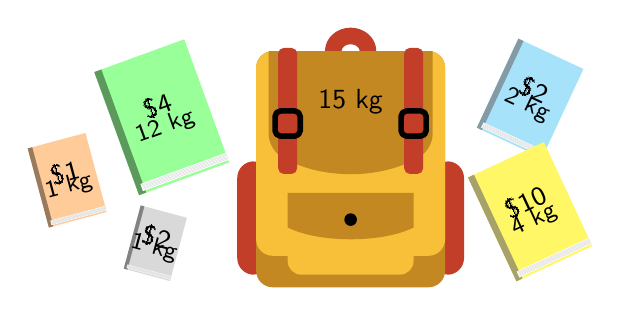
\begin{tikzpicture}[line join=round, line cap=round, font=\sffamily\footnotesize, scale=0.4]

% ---------- helpers ----------
\definecolor{bagyellow}{RGB}{248,188,46}
\definecolor{baggold}{RGB}{230,160,40}
\definecolor{bagred}{RGB}{194,62,40}

% book(pic): (x,y), angle, fill, price, weight, scale
\newcommand{\book}[7]{%
    \colorlet{bookbase}{#4}
    \colorlet{bookback}{bookbase!60!black}
    \colorlet{bookspine}{bookbase!50!white}
  \begin{scope}[shift={(#1,#2)},rotate=#3,scale=#7,]
    % cover
    \fill[rounded corners=0pt,fill=bookbase] (-1.9,-2.6) rectangle (1.9,2.6);
    \fill[rounded corners=0pt,fill=bookback] (-1.9,-2.6) rectangle (-1.6,2.6);
    % pages strip
    \fill[rounded corners=0pt,white] (-1.7,-2.5) rectangle (1.9,-2.2);
    % \draw[black!12, very thin] (-1.65,-2.45) -- (-1.65,-2.25);
    \foreach \y in {-2.45, -2.4, -2.35, -2.3, -2.25}{%
      \draw[black!12, very thin] (-1.65,\y) -- (1.9,\y);
    }
    % text
    \node[align=center,scale=1.2, rotate=#3] at (0,0.5) {\$#5};
    \node[align=center,scale=1.1, rotate=#3] at (0,-0.4) {#6 kg};
  \end{scope}%
}

% ---------- backpack ----------
% side pockets
\fill[bagred,rounded corners=6pt] (-3.6,-3) rectangle (-2.6,0.6);
\fill[bagred,rounded corners=6pt] ( 2.6,-3) rectangle ( 3.6,0.6);

% top handle
\draw[line width=6pt,bagred] (0.55,4.1) arc (0:180:0.55 and 0.48);
% \draw[line width=8pt,bagred] (0,4.1) arc (90:270:0.55 and 0.48);


% main body
\fill[baggold!85!black,rounded corners=6pt] (-3.0,-3.4) rectangle (3.0,4.1);
\fill[bagyellow!95!white,rounded corners=6pt] (-3.0,-2.4) rectangle (3.0,4.1);


% front pocket
\fill[bagyellow!95!white] (-2.0,-0.4) -- (2.0, -0.4) [rounded corners=5pt] -- (2.0,-3) [rounded corners=5pt] -- (-2, -3) [rounded corners=0pt] -- cycle;
\fill[baggold!85!black] (-2.0,-0.4) -- (2.0, -0.4)  -- (2.0,-1.5)  .. controls (1,-2) and (-1,-2) .. (-2, -1.5) -- cycle;
\fill[black] (0,-1.25) circle (0.2);

% flap
\fill[baggold!85!black] (-2.6,4.1) -- (2.6, 4.1) [rounded corners=5pt] -- (2.6, 1) .. controls (1.0, 0) and (-1, 0) .. (-2.6, 1) [rounded corners=0pt] -- cycle;


% shoulder straps + buckles
\fill[rounded corners=2pt,bagred] (-2.3,4.2) rectangle (-1.7,0.2);
\fill[rounded corners=2pt,bagred] ( 2.3,4.2) rectangle ( 1.7,0.2);
\draw[black,rounded corners=2pt, line width=2pt] (-2.4,1.4) rectangle (-1.6,2.2);
\draw[black,rounded corners=2pt, line width=2pt] ( 1.6,1.4) rectangle (2.4,2.2);

% weight label
\node[font=\sffamily] at (0,2.5) {15 kg};

% ---------- books ----------
\book{-6}{2.0}{20}{green!40}{4}{12}{0.8}
\book{-6.2}{-2.0}{-15}{gray!30}{2}{1}{0.4}
\book{-9}{0}{15}{orange!40}{1}{1}{0.5}
\book{5.7}{2.6}{-25}{cyan!35}{2}{2}{0.6}
\book{5.7}{-1.0}{25}{yellow!60}{10}{4}{0.7}

\end{tikzpicture}
\]


% \[
% \operatorname{opt}(i, w) 
% =
% \begin{cases}
% 0 & \text{if } i = 0\\
% \operatorname{opt}(i-1, w) & \text{if } w_i > w\\
% \max\{ v_i + \operatorname{opt}(i-1, w - w_i), \operatorname{opt}(i-1, w)\} & \text{otherwise}
% \end{cases}
% \]
% % where \(i\) is the index of the current item, \(w\) is the remaining weight capacity, \(w_i\) is the weight of item \(i\) and \(v_i\) is the value of item \(i\).     



\definecolor{knapblue}{RGB}{0,130,130}
\definecolor{knapred}{RGB}{180,0,0}
recursive formulation:
\[
\operatorname{opt}(i, w)
=
\left\{
\begin{array}{@{}l@{\quad}l@{\quad}l@{}}
{0}
  & {i = 0}
  & \textcolor{knapred}{\triangleright\ \text{no items left}}\\[0.3em]
{\operatorname{opt}(i-1, w)}
  & {w_i > w}
  & \textcolor{knapred}{\triangleright\ \text{item too heavy}}\\[0.3em]
{\max\{v_i + \operatorname{opt}(i-1, w - w_i),\ \operatorname{opt}(i-1, w)\}}
  & {\text{otherwise}}
  & \textcolor{knapred}{\triangleright\ \text{include or exclude item $i$?}}
\end{array}
\right.
\]



% \begin{algorithmic}[1]
% \Function{opt}{$i, w$}
%   \If{$i = 0$} \Comment{no items left}
%     \State \Return \(0\)
%   \ElsIf{$w_i > w$} \Comment{item too heavy}
%     \State \Return \Call{opt}{$i-1, w$}
%   \Else \Comment{include or exlude item \(i\)?}
%     \State \Return \(\max\{ v_i + \Call{opt}{i-1, w - w_i}, \Call{opt}{i-1, w} \}\)
%   \EndIf
% \EndFunction
% \end{algorithmic}



% \[
% \operatorname{opt}(i,w) 
% =
% \begin{cases}
% 0 & \text{if } i = 0 \text{ (no items left)}\\[0.3em]
% \operatorname{opt}(i-1, w) & \text{if } w_i > w \text{ (too heavy)}\\[0.3em]
% \max\{ v_i + \operatorname{opt}(i-1, w - w_i), \operatorname{opt}(i-1, w)\}
%   & \text{otherwise (include or exclude item $i$?)}
% \end{cases}
% \]



top down memoized:
\begin{algorithm}[h]
\caption{Knapsack (top-down, memoized)}\label{alg:knapsack_topdown}
\begin{algorithmic}[1]
\Function{Opt}{$i, w$}
  \If{\(M[i,w] = \nil\)} 
    \If{\(i = 0\)} 
    \State \(M[i,w] \gets 0\) \Comment{no items left}
    \ElsIf{\(w_i > w\)} 
    \State \(M[i,w] \gets \Call{Opt}{i-1, w}\) \Comment{item too heavy}      
    \Else 
    \State \(M[i,w] \gets \max\{ v_i + \Call{Opt}{i-1, w - w_i}, \Call{Opt}{i-1, w} \}\) \Comment{include or exclude?}
    \EndIf
  \EndIf
  \State \Return \(M[i,w]\)
\EndFunction
\end{algorithmic}
\end{algorithm}


\textcolor{AccentBlue}{Bottom-up (tabulation) version.}
Instead of recursion + memoization, we can fill a DP table iteratively.
Let \(W\) be the knapsack capacity.
We build a table \(\operatorname{OPT}[i,w]\) for \(i = 0,\ldots,n\) and \(w = 0,\ldots,W\),
where
\(
\operatorname{OPT}[i,w]
\)
denotes the maximum value achievable using items \(1,\ldots,i\) with capacity \(w\).


\begin{algorithm}[h]
\caption{Knapsack (bottom-up DP)}\label{alg:knapsack_bottomup}
\begin{algorithmic}[1]
\Require items \(1,\ldots,n\) with weights \(w_i\), values \(v_i\); capacity \(W\)
\For{$w = 0 \TO W$}
  \State \(\operatorname{OPT}[0,w] \gets 0\) \Comment{no items}
\EndFor
% \For{$i = 0 \TO n$}
%   \State \(\operatorname{OPT}[i,0] \gets 0\) \Comment{zero capacity}
% \EndFor
\For{$i = 1 \TO n$}
  \For{$w = 0 \TO W$}
    \If{$w_i > w$}
      \State \(\operatorname{OPT}[i,w] \gets \operatorname{OPT}[i-1,w]\) \Comment{item \(i\) too heavy}
    \Else
      \State \(\operatorname{OPT}[i,w] \gets
        \max\bigl\{
          v_i + \operatorname{OPT}[i-1, w - w_i],\;
          \operatorname{OPT}[i-1, w]
        \bigr\}\)
    \EndIf
  \EndFor
\EndFor
\State \Return \(\operatorname{OPT}[n,W]\)
\end{algorithmic}
\end{algorithm}

\textcolor{AccentBlue}{Running time.}
The table has \((n+1)(W+1) = O(nW)\) entries, 
and each is filled in \(O(1)\) time, so the running time is \(O(nW)\) and the space is \(O(nW)\).
By keeping only two rows at a time, the space can be reduced to \(O(W)\).

\begin{remark}
0/1 Knapsack is NP-hard in general, so we do not expect a polynomial-time algorithm in the input size.
The DP runs in time polynomial in \(n\) and \(W\), which is called \emph{pseudo-polynomial} time,
because \(W\) is exponential in the number of bits needed to represent it (i.e. the input size).
\end{remark}


\textcolor{AccentBlue}{Approximation algorithm}.
There exists a polynomial algorithm that produces a feasible solution that has value within 0.01\% of the optimum.






\subsection{Sequence Alignment}\label{sec:sequence_alignment}

\textcolor{AccentBlue}{Goal}.
Given two strings \(X = x_1x_2\cdots x_m\) and \(Y = y_1y_2\cdots y_n\),
find an {alignment of minimum total cost}.


\begin{definition}[Alignment]\label{def:alignment}
An \textcolor{AccentRed}{alignment} \(M\) between two strings \(X\) and \(Y\) is a set of ordered pairs \((x_i, y_j)\) such that each item occurs in at most one pair and no two pairs cross.
\end{definition}

\begin{definition}\label{def:cross}
Two pairs \((x_i, y_j)\) and \((x_{i'}, y_{j'})\) \textcolor{AccentRed}{cross} if \(i < i'\) but \(j > j'\).
\end{definition}

\begin{definition}[Cost Model]\label{def:cost_model}
% \textcolor{AccentBlue}{Cost model}.
Aligning \(x_i\) with \(y_j\) incurs a \emph{mismatch} penalty \(\alpha_{x_i y_j}\).
Leaving a character unmatched (aligning it with a gap ``\(-\)'') incurs a \emph{gap} penalty \(\delta > 0\).
\end{definition}
  % The \hl{edit distance} between \(X\) and \(Y\) is the minimum cost over all alignments.

\begin{definition}[Cost]\label{def:alignment_cost}
The \textcolor{AccentRed}{cost} of an alignment \(M\) is
\[
  \operatorname{cost}(M)
  =
  \underbrace{\sum_{(x_i, y_j) \in M} \alpha_{x_i y_j}}_{\text{mismatch}} 
  + 
  \underbrace{\sum_{i \colon \text{\(x_i\) unmatched}} \delta+\sum_{j \colon \text{\(y_j\) unmatched}} \delta}_{\text {gap }}
\]
i.e. it is the sum of all gap and mismatch penalties.
\end{definition}

\begin{definition}[Edit distance]\label{def:edit_distance}
The \textcolor{AccentRed}{edit distance} between strings \(X\) and \(Y\) is the minimum \nameref{def:alignment_cost} over all \nameref{def:alignment}s  
\end{definition}

\textcolor{AccentBlue}{DP formulation}.
Let
\(
\operatorname{OPT}(i,j)
\) 
denote the minimum cost of aligning the prefixes \(x_1\cdots x_i\) and \(y_1\cdots y_j\).
If either of the prefixes is empty and the other has length \(k\), the only option is to align all characters of the other prefix with gaps, incurring a cost of \(\delta\) per gap, i.e.
\(\operatorname{OPT}(k,0) = \operatorname{OPT}(0,k) = k \cdot \delta\).
Otherwise we have three choices:
\begin{itemize}
  \item Case 1: match \(x_i\) with \(y_j\): \(\alpha_{x_i y_j} + \operatorname{OPT}(i-1,j-1)\)
  \begin{itemize}
    \item[-] pay mismatch cost \(\alpha_{x_i y_j}\) plus whatever the minimum cost is for aligning the prefixes \(x_1\cdots x_{i-1}\) and \(y_1\cdots y_{j-1}\)
  \end{itemize}
  \item Case 2a: leave \(x_i\) unmatched (align with gap): \(\delta + \operatorname{OPT}(i-1,j)\)
  \begin{itemize}
    \item[-] pay gap cost \(\delta\) for \(x_i\) plus min cost for aligning \(x_1\cdots x_{i-1}\) and \(y_1\cdots y_{j}\)
  \end{itemize}
  \item Case 2b: leave \(y_j\) unmatched (align with gap): \(\delta + \operatorname{OPT}(i,j-1)\)
  \begin{itemize}
    \item[-] pay gap cost \(\delta\) for \(y_j\) plus min cost for aligning \(x_1\cdots x_{i}\) and \(y_1\cdots y_{j-1}\)
  \end{itemize}
\end{itemize}


We get the recurrence:
\begin{equation}\label{eq:sequence_alignment_recurrence}
\operatorname{OPT}(i,j)
=
\begin{cases}
j \cdot \delta & \text{if \(i = 0\)}\\
i \cdot \delta & \text{if \(j = 0\)}\\
\min
\begin{cases}
\alpha_{x_i y_j} + \operatorname{OPT}(i-1,j-1)\\
\delta + \operatorname{OPT}(i-1,j)\\
\delta + \operatorname{OPT}(i,j-1)
\end{cases}
& \text{otherwise}
\end{cases}
\end{equation}

\medskip
To compute \(\operatorname{OPT}(m,n)\):
\begin{itemize}
\item build up the values of \(\operatorname{OPT}(i,j)\) using the recurrence -- fill an \(m \times n\) table
\item \(O(mn)\) subproblems
\item to compute \(\operatorname{OPT}(i,j)\) we need: \(\operatorname{OPT}(i-1,j)\), \(\operatorname{OPT}(i-1,j-1)\), \(\operatorname{OPT}(i,j-1)\)
\item can fill table \emph{row by row} or \emph{column by column}
\item cost we are looking for will be in bottom-right cell \(\operatorname{OPT}(m,n)\)
\end{itemize}


\begin{algorithm}[h]
\caption{Sequence Alignment}\label{alg:sequence_alignment}
\begin{algorithmic}[1]
\Require strings \(X=x_1\cdots x_m\), \(Y=y_1\cdots y_n\); gap penalty \(\delta\); mismatch costs \(\alpha_{pq}\)
\For{$i = 0 \TO m$}
  \State \(M[i,0] \gets i\delta\)
\EndFor
\For{$j = 0 \TO n$}
  \State \(M[0,j] \gets j\delta\)
\EndFor
\For{$i = 1 \TO m$}
  \For{$j = 1 \TO n$}
    \State \(M[i,j] \gets \min\bigl\{\alpha_{x_i y_j}+M[i-1,j-1], \delta+M[i-1,j], \delta+M[i,j-1]\bigr\}\) \label{line:seqalign_dp_decision}
  \EndFor
\EndFor
\State \Return \(M[m,n]\)
\end{algorithmic}
\end{algorithm}

\textcolor{AccentBlue}{Running time}.
The table has \((m+1)(n+1) = O(mn)\) entries and each entry is computed in \(O(1)\),
so the running time is \(O(mn)\) and the space usage is \(O(mn)\).


\begin{remark}
We can reduce the space to \(O(\min\{m,n\})\) if only the optimal cost is needed by keeping only two rows/columns in memory at a time while ``filling the table''.
Because to compute \(M[i,j]\) we only need \(M[i-1,j-1]\), \(M[i-1,j]\), and \(M[i,j-1]\).
\end{remark}


\textcolor{AccentBlue}{Recovering an optimal alignment}.
Two options:
\begin{itemize}
\item Do a postprocessing step after filling the table:
Starting at \((m,n)\), backtrack to \((0,0)\) by comparing \(M[i,j]\) with the three candidate predecessors:
\((i-1,j-1)\), \((i-1,j)\), \((i,j-1)\).
Record the corresponding aligned characters (\(x_i\) vs. \(y_j\), \(x_i\) vs. ``\(-\)'', or ``\(-\)'' vs. \(y_j\)).
Ties correspond to multiple optimal alignments.
\item Store another array (hint table):
Every time we make a decision in \autoref{line:seqalign_dp_decision} of \autoref{alg:sequence_alignment}, 
keep a hint of where we came from.
\end{itemize}


% \clearpage










\subsection{Longest Common Subsequence} \label{sec:lcs}
Let us think of character strings as sequences of characters. 
Given $X=\left\langle x_1, \ldots, x_l\right\rangle$, we say that $Z=\left\langle z_1, \ldots, z_k\right\rangle$ is a subsequence of $X$ if there is a strictly increasing sequence of $k$ indices $\left\langle i_1, \ldots, i_k\right\rangle$ such that $Z=\left\langle x_{i_1}, \ldots, x_{i_k}\right\rangle$. 

Given two strings \(X=\left\langle x_1, \ldots, x_m\right\rangle\) and \(Y = \left\langle y_1, \ldots, y_n \right\rangle\), the longest common subsequence of $X$ and $Y$ is a longest sequence $Z$ that is a subsequence of both $X$ and $Y$. 

\subsubsection{Brute force}
A brute force approach would be to enumerate all subsequences of $X$ and check for each whether it is also a subsequence of $Y$. 
There are $2^m$ subsequences of \(X\) and checking wether it is a subsequence of \(Y\) takes \(O(n)\) time:
Scan \(Y\) for first occurence, from there scan for second, and so on.
In total this takes \(\Theta(n 2^m)\) time.


\subsubsection{Dynamic programming formulation}
A prefix \(X_i\) of a sequence \(X\) is just an initial string of values, \(X_i = \langle x_1, \ldots, x_i \rangle\).
\(X_0\) is the empty sequence.
The idea is to compute the longest common subsequence for every possible pair of prefixes (there are \(O(mn)\) such pairs).

Let $\operatorname{lcs}(i, j)$ denote the length of the longest common subsequence of $X_i$ and $Y_j$.
We have the following recursive relation:
\[
\operatorname{lcs}(i, j)
= 
\begin{cases}
  0 & \text { if } i=0 \text { or } j=0 \\ 
  \operatorname{lcs}(i-1, j-1)+1 & \text { if } i, j>0 \text { and } x_i=y_j \\ 
  \max (\operatorname{lcs}(i-1, j), \operatorname{lcs}(i, j-1)) & \text { if } i, j>0 \text { and } x_i \neq y_j
\end{cases}
\]


Last characters match:
\[
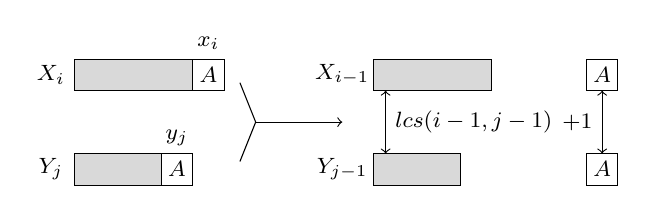
\begin{tikzpicture}[scale=0.5, font=\footnotesize]

%--- left strings Xi, Yj ------------------------------------------
% Xi row
\node at (0,1.2) {$X_i$};
\draw[fill=gray!30] (0.6,0.8) rectangle (3.6,1.6);   % prefix of Xi
\draw              (3.6,0.8) rectangle (4.4,1.6);     % last char
\node at (4.0,1.2) {$A$};
\node at (4.0,2.0) {$x_i$};

% Yj row
\node at (0,-1.2) {$Y_j$};
\draw[fill=gray!30] (0.6,-1.6) rectangle (2.8,-0.8);  % prefix of Yj
\draw              (2.8,-1.6) rectangle (3.6,-0.8);   % last char
\node at (3.2,-1.2) {$A$};
\node at (3.2,-0.4) {$y_j$};

%--- branching + arrow --------------------------------------------
\coordinate (c) at (5.2,0);
\draw (4.8,1.0) -- (c) -- (4.8,-1.0);
\draw[->] (c) -- (7.4,0);

%--- right strings Xi-1, Yj-1 -------------------------------------
% Xi-1 row
\node at (7.4,1.2) {$X_{i-1}$};
\draw[fill=gray!30] (8.2,0.8) rectangle (11.2,1.6);

% Yj-1 row
\node at (7.4,-1.2) {$Y_{j-1}$};
\draw[fill=gray!30] (8.2,-1.6) rectangle (10.4,-0.8);
% vertical lcs arrow and label
\draw[<->] (8.5,0.8) -- (8.5,-0.8);
\node[right] at (8.5,0) {$\operatorname{lcs}(i-1,j-1)$};

%--- "+1" and two A boxes -----------------------------------------
\node[left] at (14,0) {$+1$};

\draw (13.6,0.8)  rectangle (14.4,1.6);
\draw (13.6,-1.6) rectangle (14.4,-0.8);
\node at (14.0,1.2) {$A$};
\node at (14.0,-1.2) {$A$};
\draw[<->] (14.0,0.8) -- (14.0,-0.8);

\end{tikzpicture}
\]


Last characters do not match:
\[
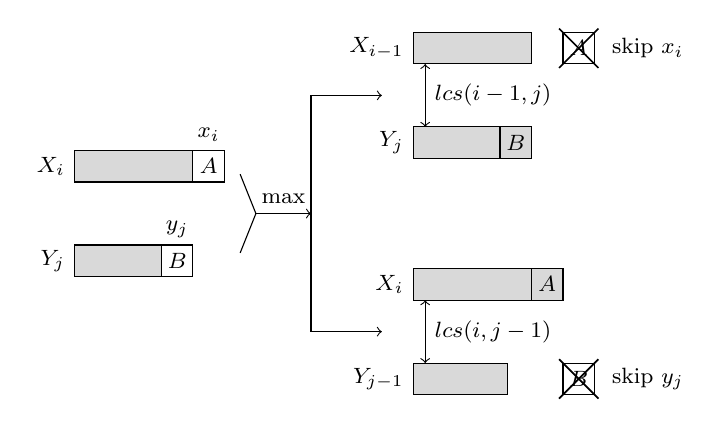
\begin{tikzpicture}[scale=0.5, font=\footnotesize]

%--- left strings Xi, Yj ------------------------------------------
% Xi row
\node[left] at (0.6,1.2) {$X_i$};
\draw[fill=gray!30] (0.6,0.8) rectangle (3.6,1.6);   % prefix of Xi
\draw              (3.6,0.8) rectangle (4.4,1.6);     % last char
\node at (4.0,1.2) {$A$};
\node at (4.0,2.0) {$x_i$};

% Yj row
\node[left] at (0.6,-1.2) {$Y_j$};
\draw[fill=gray!30] (0.6,-1.6) rectangle (2.8,-0.8);  % prefix of Yj
\draw              (2.8,-1.6) rectangle (3.6,-0.8);   % last char
\node at (3.2,-1.2) {$B$};
\node at (3.2,-0.4) {$y_j$};

%--- branching + arrow --------------------------------------------
\coordinate (c) at (5.2,0);
\draw (4.8,1.0) -- (c) -- (4.8,-1.0);
\draw[->] (c) -- (6.6,0);
\node[above] at (5.9,0) {$\max$};
\draw (6.6,3.0) -- (6.6,-3.0);
\draw[->] (6.6,3) -- (8.4,3);
\draw[->] (6.6,-3) -- (8.4,-3);


\begin {scope}[shift={(1, 3)}]
%--- right strings Xi-1, Yj-1 -------------------------------------
% Xi-1 row
\node[left] at (8.2,1.2) {$X_{i-1}$};
\draw[fill=gray!30] (8.2,0.8) rectangle (11.2,1.6);

\draw (12,0.8) rectangle (12.8,1.6);
\node at (12.4,1.2) {$A$};

% cross
\draw[line width=0.6pt] (11.9,0.7) -- (12.9,1.7);
\draw[line width=0.6pt] (11.9,1.7) -- (12.9,0.7);
\node[right] at (13,1.2) {skip $x_i$};

% Yj-1 row
\node[left] at (8.2,-1.2) {$Y_{j}$};
\draw[fill=gray!30] (8.2,-1.6) rectangle (10.4,-0.8);
\draw[fill=gray!30] (10.4,-1.6) rectangle (11.2,-0.8);
\node at (10.8,-1.2) {$B$};
% vertical lcs arrow and label
\draw[<->] (8.5,0.8) -- (8.5,-0.8);
\node[right] at (8.5,0) {$\operatorname{lcs}(i-1,j)$};
\end{scope}

\begin {scope}[shift={(1, -3)}]
%--- right strings Xi-1, Yj-1 -------------------------------------
% Xi-1 row
\node[left] at (8.2,1.2) {$X_{i}$};
\draw[fill=gray!30] (8.2,0.8) rectangle (11.2,1.6);
\draw[fill=gray!30] (11.2,0.8) rectangle (12.0,1.6);
\node at (11.6,1.2) {$A$};

% Yj-1 row
\node[left] at (8.2,-1.2) {$Y_{j-1}$};
\draw[fill=gray!30] (8.2,-1.6) rectangle (10.6,-0.8);

\draw (12.0,-1.6) rectangle (12.8,-0.8);
\node at (12.4,-1.2) {$B$};

% cross
\draw[line width=0.6pt] (11.9,-1.7) -- (12.9,-0.7);
\draw[line width=0.6pt] (11.9,-0.7) -- (12.9,-1.7);
\node[right] at (13, -1.2) {skip $y_j$};


% vertical lcs arrow and label
\draw[<->] (8.5,0.8) -- (8.5,-0.8);
\node[right] at (8.5,0) {$\operatorname{lcs}(i,j-1)$};
\end{scope}


\end{tikzpicture}
\]





\textcolor{AccentBlue}{DP table.}
We store values in a table \(L[0\ldots m, 0\ldots n]\) where
\(L[i,j] = \operatorname{lcs}(i,j)\).
We can go recursive/top-down with memoization (\autoref{alg:lcs_topdown}) or iterative/bottom-up (\autoref{alg:lcs}).


\begin{algorithm}[h]
\caption{Longest Common Subsequence (top-down DP)} \label{alg:lcs_topdown}
\begin{algorithmic}[1]
\Function{LCS}{$i, j$}
  \If{\(L[i,j] = \nil\)}
    \If{\(i = 0 \OR j = 0\)} \Comment{base case}
      \State \(L[i,j] \gets 0\)
    \ElsIf{\(x_i = y_j\)} \Comment{last characters match}
      \State \(L[i,j] \gets \Call{LCS}{i-1, j-1} + 1\)
    \Else \Comment{last characters do not match}
      \State \(L[i,j] \gets \max\{\Call{LCS}{i-1, j}, \Call{LCS}{i, j-1}\}\)
    \EndIf
  \EndIf
  \State \Return \(L[i,j]\) \Comment{return stored value}
\EndFunction
\end{algorithmic}
\end{algorithm}


\begin{algorithm}[h]
\caption{Longest Common Subsequence (bottom-up DP)}\label{alg:lcs}
\begin{algorithmic}[1]
\Require strings \(X = x_1\cdots x_m\), \(Y = y_1\cdots y_n\)
\State \(L \gets \text{new array \([0 \ldots m, 0 \ldots n]\)}\)
\For{$i = 0 \TO m$}
  \State \(L[i,0] \gets 0\)
\EndFor
\For{$j = 0 \TO n$}
  \State \(L[0,j] \gets 0\)
\EndFor
\For{$i = 1 \TO m$} \Comment{iterate over rows}
  \For{$j = 1 \TO n$} \Comment{iterate over columns}
    \If{$x_i = y_j$} 
      \State \(L[i,j] \gets L[i-1,j-1] + 1\) \Comment{take \(x_i = y_j\) for LCS}
    \Else
      \State \(L[i,j] \gets \max\{L[i-1,j], L[i,j-1]\}\)
    \EndIf
  \EndFor
\EndFor
\State \Return \(L[m,n]\)
\end{algorithmic}
\end{algorithm}




\textcolor{AccentBlue}{Running time} of \autoref{alg:lcs}.
The table has \((m+1)(n+1) = O(mn)\) entries, each filled in \(O(1)\) time,
so the running time is \(O(mn)\) and the space is \(O(mn)\).




\subsubsection{Reconstructing the actual subsequence}

To retrieve the actual subsequence, we can use another table, a ``hint'' table \(h[0\ldots m, 0\ldots n]\) that records which of the three cases was used to compute each \(L[i,j]\) (\autoref{alg:lcs_with_hints}).

\begin{algorithm}[h]
\caption{LCS (bottom-up) with hints}\label{alg:lcs_with_hints}
\begin{algorithmic}[1]
\Require strings \(X = x_1\cdots x_m\), \(Y = y_1\cdots y_n\)
\State \(L \gets \text{new array \([0 \ldots m, 0 \ldots n]\)}\) \Comment{stores lcs lengths}
\State \(h \gets \text{new array \([0 \ldots m, 0 \ldots n]\)}\) \Comment{hint table}
\For{$i = 0 \TO m$} \Comment{initialize column 0}
  \State \(L[i,0] \gets 0\)
  \State \(h[i,0] \gets \text{skipX}\)
\EndFor
\For{$j = 0 \TO n$} \Comment{initialize row 0}
  \State \(L[0,j] \gets 0\)
  \State \(h[0,j] \gets \text{skipY}\)
\EndFor
\For{$i = 1 \TO m$}
  \For{$j = 1 \TO n$}
    \If{$x_i = y_j$}
      \State \(L[i,j] \gets L[i-1,j-1] + 1\)
      \State \(h[i,j] \gets \text{addXY}\)
    \Else
      \If{$L[i-1,j] \ge L[i,j-1]$}
        \State \(L[i,j] \gets L[i-1,j]\)
        \State \(h[i,j] \gets \text{skipX}\)
      \Else
        \State \(L[i,j] \gets L[i,j-1]\)
        \State \(h[i,j] \gets \text{skipY}\)
      \EndIf
    \EndIf
  \EndFor
\EndFor
\State \Return \(L[m,n]\), \(h\)
\end{algorithmic}
\end{algorithm}


Now we can use the hints to reconstruct the LCS:
\begin{itemize}
  \item start at the last entry of the table, \([m,n]\)
  \item if \(h[i,j] = \text{addXY}\) (\(\nwarrow\)), then \(x_i = y_j\) is appended to LCS, continue with \([i-1,j-1]\)
  \item if \(h[i,j] = \text{skipX}\) (\(\uparrow\)), then \(x_i\) is not in LCS, continue with \([i-1,j]\)
  \item if \(h[i,j] = \text{skipY}\) (\(\leftarrow\)), then \(y_j\) is not in LCS, continue with \([i,j-1]\)
  \item stop when reaching \([0,0]\)
\end{itemize}

Because the characters are generated in revers order, prepend them to a sequence, so that when we are done, the sequence is in correct order.
Or use recursion to print them in correct order directly (\autoref{alg:print_lcs}).

\begin{algorithm}[h]
\caption{recursive LCS printing using hints}\label{alg:print_lcs}
\begin{algorithmic}[1]
\Function{Print-LCS}{$h, X, i, j$}
  \If{\(i = 0 \OR j = 0\)}
    \State \Return
  \EndIf
  \If{\(h[i,j] = \text{addXY}\)}
    \State \Call{Print-LCS}{$h, X, i-1, j-1$}
    \State {print} \(x_i\)
  \ElsIf{\(h[i,j] = \text{skipX}\)}
    \State \Call{Print-LCS}{$h, X, i-1, j$}
  \Else
    \State \Call{Print-LCS}{$h, X, i, j-1$}
  \EndIf
\EndFunction
\end{algorithmic}
\end{algorithm}





Alternatively, the hints can be discovered based on the filled \(L\) table (\autoref{alg:print_lcs_discovered}, \autoref{alg:print_lcs_discovered_alt}).
If \(x_i = y_j\) and \(L[i,j] = L[i-1,j-1]+1\), then \(x_i\) is part of some LCS and we move to \([i-1,j-1]\); 
otherwise, if \(L[i-1,j] \ge L[i,j-1]\) move to \([i-1,j]\), else move to \([i,j-1]\).


\begin{algorithm}[h]
\caption{recursive LCS printing discovering hints}\label{alg:print_lcs_discovered}
\begin{algorithmic}[1]
\Function{Print-LCS}{$L, X, Y, i, j$}
  \If{\(i = 0 \OR j = 0\)}
    \State \Return
  \EndIf
  \If{\(x_i = y_j \AND L[i,j] = L[i-1,j-1]+1\)}
    \State \Call{Print-LCS}{$L, X, Y, i-1, j-1$} \Comment{take \(x_i = y_j\)}
    \State {print} \(x_i\)
  \ElsIf{\(L[i-1,j] \ge L[i,j-1]\)}
    \State \Call{Print-LCS}{$L, X, Y, i-1, j$} \Comment{skip \(x_i\)}
  \Else
    \State \Call{Print-LCS}{$L, X, Y, i, j-1$} \Comment{skip \(y_j\)}
  \EndIf
\EndFunction
\end{algorithmic}
\end{algorithm}


\begin{algorithm}[h]
\caption{recursive LCS printing discovering hints (alternative condition)}\label{alg:print_lcs_discovered_alt}
\begin{algorithmic}[1]
\Function{Print-LCS}{$L, X, i, j$}
  \If{\(i = 0 \OR j = 0\)}
    \State \Return
  \EndIf
  \If{\(L[i,j] = L[i-1,j]\)}
    \State \Call{Print-LCS}{$L, X, i-1, j$} \Comment{move up i.e. skip \(x_i\)}
  \ElsIf{\(L[i,j] = L[i,j-1]\)}
    \State \Call{Print-LCS}{$L, X, i, j-1$} \Comment{move left i.e. skip \(y_j\)}
  \Else \Comment{\(L[i,j]\) must be different from all 3 neighbors, so \(x_i = y_j\)}
    \State \Call{Print-LCS}{$L, X, i-1, j-1$} \Comment{move diagonally, take \(x_i = y_j\)}
    \State {print} \(x_i\)
  \EndIf
\EndFunction
\end{algorithmic}
\end{algorithm}

 \autoref{alg:print_lcs}, \autoref{alg:print_lcs_discovered} and \autoref{alg:print_lcs_discovered_alt} are called with initial parameters \(i = m\) and \(j = n\).




\begin{remark}
Again, we can reduce the space to \(O(\min\{m,n\})\) if only the length of the LCS is needed by keeping only two rows/columns in memory at a time while ``filling the table''.
Because to compute \(L[i,j]\) we only need \(L[i-1,j-1]\), \(L[i-1,j]\), and \(L[i,j-1]\).
\end{remark}



\subsection{Sequence Alignment in linear space}\label{sec:seqalign_lcs_linear_space}
There is a cool trick that allows linear space without compromising the time complexity asymptotically.
It combines Dynamic Programming with Divide and Conquer.
The same trick can be used for \nameref{sec:lcs}.

Can we avoid using quadratic space?

\textcolor{AccentBlue}{easy:} \textcolor{AccentRed}{optimal value}: \(O(m + n)\) space and \(O(mn)\) time.
\begin{itemize}
  \item use a \(2 \times n\) matrix. compute \(\operatorname{OPT}(i, \cdot)\) from \(\operatorname{OPT}(i-1, \cdot)\)
  \item but no longer a simple way to recover the alignment itself
\end{itemize}

\begin{theorem}[Hirschberg 1975]\label{thm:hirschberg}
Optimal alignment in \(O(m + n)\) space and \(O(mn)\) time. Clever combination of divide-and-conquer and dynamic programming.
\end{theorem}

A DP matrix can be seen as a directed acyclic graph (DAG).
The optimal alignment corresponds to the shortest path in the DAG from node \((0,0)\) to \((m,n)\).

\textcolor{AccentBlue}{Edit distance graph}:
Add a node for every entry \(M[i,j]\) and an edge from \(M[i-1,j-1]\), \(M[i-1,j]\), \(M[i,j-1]\) to \(M[i,j]\) with weights according the \nameref{def:cost_model}:
\[
\begin{tikzpicture}[
  scale=1.5,
  font=\footnotesize,
  dpnode/.style={circle, minimum size=3mm, inner sep=0pt, draw=gray!60, fill=gray!20},
  startend/.style={dpnode, minimum size=6mm, draw=black, fill=none},
  focus/.style={dpnode, minimum size=6mm, draw=black, fill=red!20},
  ed/.style={-Latex, draw=gray!55, line width=0.6pt},
  edD/.style={ed, densely dotted}, % dashed "collapsed" connections
  edF/.style={ed, color=black}
]

% --- nodes (create ALL nodes once, with correct style/label)
\foreach \r in {0,1,2,3,4,5}{
  \foreach \c in {0,1,2,3,4,5,6,7}{
    \def\nodestyle{dpnode}
    \def\nodelabel{}%

    % special nodes (same names!)
    \ifnum\r=0 \ifnum\c=0 \def\nodestyle{startend}\def\nodelabel{$0$-$0$}\fi\fi
    \ifnum\r=3 \ifnum\c=4 \def\nodestyle{focus}\def\nodelabel{$i$-$j$}\fi\fi
    \ifnum\r=5 \ifnum\c=7 \def\nodestyle{startend}\def\nodelabel{$m$-$n$}\fi\fi

    \node[\nodestyle] (n\r\c) at (\c,-\r) {\nodelabel};
  }
}

% ---- horizontal edges (skip n33 -> n34)
\foreach \r in {0,1,2,3,4,5}{
  \foreach \c in {0,1,2,3,4,5,6}{
    \pgfmathtruncatemacro{\cp}{\c+1}

    % choose style
    \def\estyle{ed}
    \ifnum\c=2 \def\estyle{edD}\fi
    \ifnum\c=4 \def\estyle{edD}\fi

    % skip only if (r,c)=(3,3)
    \ifnum\r=3
      \ifnum\c=3
        % skip
      \else
        \draw[\estyle] (n\r\c) -- (n\r\cp);
      \fi
    \else
      \draw[\estyle] (n\r\c) -- (n\r\cp);
    \fi
  }
}

% ---- vertical edges (skip n24 -> n34)
\foreach \r in {0,1,2,3,4}{
  \pgfmathtruncatemacro{\rp}{\r+1}
  \foreach \c in {0,1,2,3,4,5,6,7}{

    % choose style
    \def\estyle{ed}
    \ifnum\r=1 \def\estyle{edD}\fi
    \ifnum\r=3 \def\estyle{edD}\fi

    % skip only if (r,c)=(2,4)
    \ifnum\r=2
      \ifnum\c=4
        % skip
      \else
        \draw[\estyle] (n\r\c) -- (n\rp\c);
      \fi
    \else
      \draw[\estyle] (n\r\c) -- (n\rp\c);
    \fi
  }
}

% ---- diagonal edges (skip n23 -> n34)
\foreach \r in {0,1,2,3,4}{
  \pgfmathtruncatemacro{\rp}{\r+1}
  \foreach \c in {0,1,2,3,4,5,6}{
    \pgfmathtruncatemacro{\cp}{\c+1}

    % choose style
    \def\estyle{ed}
    \ifnum\r=1 \def\estyle{edD}\fi
    \ifnum\r=3 \def\estyle{edD}\fi
    \ifnum\c=2 \def\estyle{edD}\fi
    \ifnum\c=4 \def\estyle{edD}\fi

    % skip only if (r,c)=(2,3)
    \ifnum\r=2
      \ifnum\c=3
        % skip
      \else
        \draw[\estyle] (n\r\c) -- (n\rp\cp);
      \fi
    \else
      \draw[\estyle] (n\r\c) -- (n\rp\cp);
    \fi
  }
}

% ---- highlighted incoming edges into (i,j) = n34
\draw[edF] (n24) -- node[midway, right] {$\delta$} (n34);                 % (i-1,j)
\draw[edF] (n33) -- node[midway, above] {$\delta$} (n34);                 % (i,j-1)
\draw[edF] (n23) -- node[pos=0.42, above, inner sep=0pt, outer sep=0pt, anchor=south west] {$\alpha_{x_i y_j}$} (n34); % (i-1,j-1)


\node[above=2.5mm] at (n00) {$\varepsilon$};
\node[left=2.5mm]  at (n00)  {$\varepsilon$};

\node[above=2.5mm] at (n01) {$ y_1$};
\node[above=2.5mm] at (n02) {$ y_2$};
\node[above=2.5mm] at (n03) {$ y_{j-1}$};
\node[above=2.5mm] at (n04) {$ y_j$};
\node[above=2.5mm] at (n05) {$ y_{n-2}$};
\node[above=2.5mm] at (n06) {$ y_{n-1}$};
\node[above=2.5mm] at (n07) {$ y_n$};

\node[left=2.5mm] at (n10) {$ x_1$};
\node[left=2.5mm] at (n20) {$ x_{i-1}$};
\node[left=2.5mm] at (n30) {$ x_i$};
\node[left=2.5mm] at (n40) {$ x_{m-1}$};
\node[left=2.5mm] at (n50) {$ x_m$};

% ---- pünktchen on axes at the collapsed gaps
\node[above=2.5mm] at ($(n02)!0.5!(n03)$) {$\cdots$};
\node[above=2.5mm] at ($(n04)!0.5!(n05)$) {$\cdots$};

\node[left=2.5mm]  at ($(n10)!0.5!(n20)$) {$\vdots$};
\node[left=2.5mm]  at ($(n30)!0.5!(n40)$) {$\vdots$};

\end{tikzpicture}
\]


Let \(f(i,j)\) be the (length of) shortest path from \((0,0)\) to \((i,j)\) and \(g(i,j)\) be the (length of) shortest path from \((i,j)\) to \((m,n)\).
\begin{observation}\label{obs:length_shortest_path_equals_opt}
 \(f(i,j) = M[i,j] = \operatorname{OPT}(i,j)\). 
\end{observation}
\begin{observation}\label{obs:opt_decomposition_node_on_shortest_path}
Let \(P\) be the shortest path from \((0,0)\) to \((m,n)\).
Then 
\begin{equation}\label{eq:opt_decomposition_node_on_shortest_path}
\operatorname{OPT}(m,n) = f(i,j) + g(i,j)
\end{equation}
for any node \((i,j)\) that lies on the path \(P\).
\end{observation}


\begin{observation}[Computing \(f(\cdot, j)\)]\label{obs:compute_f}
Given a column \(j\), we can compute the value of \(f(\cdot, j)\) = \(\operatorname{OPT}[\cdot, j]\) in \(O(mn)\) time and \(O(m + n)\) space.
\begin{itemize}
  \item[-] run space efficient sequence alignment to compute \(\operatorname{OPT}(m,n)\)
  \item[-] keep the entries of column \(j\) in a separate array
  \qedhere
\end{itemize}
\end{observation}

We can compute \(g(i,j)\) by reversing the edge orientations (formula indices) and inverting the roles of \((0,0)\) and \((m,n)\).
\begin{itemize}
  \item[-] we start with \(g(m,n) = 0\) and reverse indices in the recursive formula \eqref{eq:sequence_alignment_recurrence} for \(\operatorname{OPT}(i,j)\)
\end{itemize}

\medskip

The backward function \(g(i,j)\):
\begin{itemize}
  \item \(g(m,n) = 0\)
  \item \(g(m,j) = (n-j) \cdot \delta\); \(g(i,n) = (m-i) \cdot \delta\)
  \item substitute \(i-1\) by \(i+1\) and \(j-1\) by \(j+1\) in \eqref{eq:sequence_alignment_recurrence} for \(\operatorname{OPT}(i,j)\)
\end{itemize}

\begin{observation}[Computing \(g(\cdot, j)\)]\label{obs:compute_g}
Given a column \(j\), we can compute the values of \(g(\cdot, j)\) in \(O(mn)\) time and \(O(m + n)\) space.
\begin{itemize}
  \item[-] run space efficient sequence alignment to compute \(\operatorname{OPT}(0,0)\), (reversing the role of nodes \((m,n)\) and \((0,0)\) and reversing indices) 
  \item[-] keep the entries of column \(j\) in a separate array
  \qedhere
\end{itemize}
\end{observation}


Given a column \(j\), compute \(f(\cdot, j) + g(\cdot, j)\) in a separate array for all \(i\) (i.e. the entire column).
Let \(q\) be the index of the minimum
\begin{equation}\label{eq:q_minimizing_f_plus_g}
{\color{Red}\boxed{\color{black}
q \coloneq \argmin_{i \in [1 \ldots m]} \bigl(f(i,j) + g(i,j)\bigr)
}}
\end{equation}
then 
\begin{equation}\label{eq:f_plus_g_equals_opt}
{\color{Red}\boxed{\color{black}
f(q,j) + g(q,j) = \operatorname{OPT}(m,n)
}}
\end{equation}
i.e. we have found one pair $x_q$-$y_j$ (alignment \(x_q\)-\(y_j\) / \(x_q\)-gap / \(y_j\)-gap) in \(O(mn)\) time and \(O(m + n)\) space! % :-)

\medskip

Now we just need to put everything together using divide and conquer principle:
\begin{itemize}
  \item Divide \& Conquer: choose column \(j = n/2\)
  \item Compute \(f(\cdot, n/2)\). Compute \(g(\cdot, n/2)\). Compute \(f(\cdot, n/2) + g(\cdot, n/2)\)
  \item Let \(q\) be an index that minimizes \(f(i,n/2) + g(i,n/2)\)
  \item Store the pair \(x_q\)-\(y_{n/2}\) (possible alignment \(x_q\)-\(y_{n/2}\) / \(x_q\)-gap / \(y_{n/2}\)-gap)
  \item Recurse for \(X[1\ldots q]\), \(Y[1\ldots n/2]\) (top left subproblem) and \(X[q \ldots m]\), \(Y[n/2 \ldots n]\) (bottom right subproblem)
\end{itemize}

\medskip


\textcolor{AccentBlue}{Divide}:
Compute \(f(i,n/2)\) and \(g(i,n/2)\), for all \(i\), using two space-efficient DP algorithms (\autoref{obs:compute_f} and \autoref{obs:compute_g}) in \(O(mn)\) time and \(O(m+n)\) space.
\begin{itemize}
  \item find the index \(q\) that minimizes \(f(i, n/2) + g(i, n/2)\)
  \item store pair \(x_q\)-\(y_{n/2}\) (align \(x_q\)-\(y_{n/2}\) or \(x_q\)-gap or \(y_{n/2}\)-gap)
\end{itemize}

\smallskip
\textcolor{AccentBlue}{Conquer}:
recursively compute optimal alignment in top left and bottom right pieces.



\begin{algorithm}[h]
\caption{Divide-and-Conquer-Alignment (linear space)}
\label{alg:divide_and_conquer_alignment}
\begin{algorithmic}[1]
\Function{Divide-and-Conquer-Alignment}{$X,Y$}
  \State \(m \gets |X|\) \Comment{number of symbols in \(X\)}
  \State \(n \gets |Y|\) \Comment{number of symbols in \(Y\)}
  \If{\(m \le 2 \OR n \le 2\)}
    \State compute optimal alignment using \textsc{Alignment}(\(X,Y\))
  \EndIf
  \State \Call{Forward-Space-Efficient-Alignment}{\(X,Y[1:n/2]\)} \Comment{array \(f(\cdot,n/2)\)} \label{line:forward_alignment}
  \State \Call{Backward-Space-Efficient-Alignment}{\(X,Y[n/2 : n]\)} \Comment{array \(g(\cdot,n/2)\)} \label{line:backward_alignment}
  \State \(q \gets \argmin_{i \in [1 \ldots m]} \bigl(f(i,n/2) + g(i,n/2)\bigr)\) \Comment{applying \eqref{eq:q_minimizing_f_plus_g}}
  \State add pair \((q,n/2)\) to global list \(P\)
  \State \Call{Divide-and-Conquer-Alignment}{\(X[1:q],Y[1:n/2]\)} \label{line:recurse_top_left}
  \State \Call{Divide-and-Conquer-Alignment}{\(X[q:m],Y[n/2:n]\)} \label{line:recurse_bottom_right}
  \State \Return \(P\)
\EndFunction
\end{algorithmic}
\end{algorithm}

What is the running time of \autoref{alg:divide_and_conquer_alignment}?
For sure it takes at least as long as \autoref{alg:sequence_alignment} because we need to compute \(f(\cdot, n/2)\) and \(g(\cdot, n/2)\) at each level of recursion.


Let \(T(m,n)\) be the maximum running time of \autoref{alg:divide_and_conquer_alignment} on strings \(X\) and \(Y\) of length \(m\) and \(n\).
Then
\[
T(m,n) = \underbrace{T(q,n/2)}_{\text{Line~\ref{line:recurse_top_left}}} + \underbrace{T(m-q,n/2)}_{\text{Line~\ref{line:recurse_bottom_right}}} + \underbrace{O(mn)}_{\text{Lines~\ref{line:forward_alignment},\ref{line:backward_alignment}}}
\]
for some \(q \in [1 \ldots m]\) (see \autoref{eq:q_minimizing_f_plus_g}). 
We can also upper bound \(T(m,n)\) as
\[
T(m,n) \le 2 T(m,n/2) + O(mn) \overset{\text{\eqref{eq:master_theorem}}}\implies T(m,n) = O(mn \log n) 
\]
but this analysis is not tight, actually \(T(m,n) = O(mn)\).
We increase time by only a constant factor.
But we reuse space during recursive calls.



\begin{theorem}
\(T(m,n) = O(mn)\).
\end{theorem}
\begin{proof}[Induction on \(n\)]
Choose a constant \(c > 0\) such that
\begin{align}
T(m, 2) &\le cm \label{eq:DaC_base_case_m}\\
T(2, n) &\le cn \label{eq:DaC_base_case_n}\\
T(m, n) &\le cmn + T(q, n/2) + T(m-q, n/2) \label{eq:DaC_recurrence}
\end{align}
for all \(m,n \ge 1\) and all \(q \in [1 \ldots m]\).

\medskip

We prove by induction on \(n\) the statement
\[
P(n): \quad T(m,n) \le 2cmn \quad \forall m \ge 1
\]

\begin{enumerate}[label=(\roman*)]\label{proof:time_complexity_divide_and_conquer_alignment}
\item \textbf{Base cases:}
If \(m = 2\) or \(n = 2\), then by \eqref{eq:DaC_base_case_m} and \eqref{eq:DaC_base_case_n} we have
\[
T(m,n) \le \max\{cm,cn\} \le 2cmn
\quad
\text{\textcolor{Green}{\ding{52}}}
\]

\item \textbf{Induction hypothesis:}
Assume \(P(\tilde n)\) holds for all \(\tilde n < n\), i.e.
\[
T(\tilde m, \tilde n) \le 2 c \tilde m \tilde n
\]
for all \(\tilde m \ge 1\) and all \(\tilde n < n\).
\label{proof:time_complexity_divide_and_conquer_alignment:induction_hypothesis}

\item \textbf{Induction step:}
Fix any \(m \ge 1\). Then
\[
\begin{aligned}
T(m,n)
&\overset{\text{\eqref{eq:DaC_recurrence}}}\le cmn + T(q,n/2) + T(m-q,n/2)\\
&\overset{\text{\ref{proof:time_complexity_divide_and_conquer_alignment:induction_hypothesis}}}{%
\le}
cmn +
2c\cdot q\cdot \frac n2 + 2c\cdot (m-q)\cdot \frac n2\\
&= 
cmn +
cqn + c(m-q)n\\
&=
cmn +
cmn\\
&= 2cmn \quad \text{\textcolor{Green}{\ding{52}}}
\end{aligned}
\]
Since \(m\) was arbitrary, this proves \(P(n)\).
\end{enumerate}

Hence \(T(m,n) = O(mn)\).
\end{proof}

























\pagebreak[3]
\subsection{Shortest Paths with Negative Weights}



For graphs with possibly negative edge weights (but no negative-weight cycles reachable from the source),
\nameref{alg:dijkstra}'s greedy algorithm no longer works.
% The \nameref{alg:bellmanford} algorithm is a dynamic-programming, label-correcting method that works for arbitrary real edge weights and detects negative-weight cycles.






\begin{caution}
It may be tempting to use \nameref{alg:dijkstra} with negative weights by adding a constant to all edge weights to make them non-negative.
However, this approach does not preserve shortest paths (the new shortest paths may differ from the original ones).
\end{caution}


\begin{observation}\label{obs:negative_cost_cycle}
If some path from \(s\) to \(t\) contains a negative cost cycle,
then there does not exist a well-defined shortest \(s\)-\(t\) path (cost can be made arbitrarily small by traversing the negative cycle multiple times).
If there is no negative cost cycle, the shortest path is simple (no cycle) and has at most \(n-1\) edges
(otherwise some vertex would be repeated, forming a cycle that could be removed to yield a shorter path).
\end{observation}


% We want to find a recursive DP formulation for the cost of shortest path from a node \(v\) to the target \(t\) (equiv. from the source \(s\) to a node \(v\)).

Recursively formulate \(\operatorname{OPT}(v, ?)\): length of shortest \(v\)-\(t\) path.
\begin{itemize}
  \item Think of a parameter to facilitate the recursive formulation of a shortest path.
  \item Idea: use number of edges \(i\).
\end{itemize}
\begin{notation}
\(\operatorname{OPT}(i, v)
\coloneq
\text{length of shortest \(v\)-\(t\) path \(P\) using \emph{at most} \(i\) edges}\).
\end{notation}


compute \(\operatorname{OPT}(n-1,v)\) for every node \(v\).

\textcolor{AccentBlue}{Goal}: \(\operatorname{OPT}(n-1,s)\)

\medskip

We need to distinguish the following cases:
\begin{itemize}
  \item Case 1: \(P\) uses \(< i\) (\(\le i-1\)) edges: \(\operatorname{OPT}(i, v) = \operatorname{OPT}(i-1, v)\)
  \item Case 2: \(P\) uses exactly \(i\) edges.
  \begin{itemize}
  \item[-] 
  Let \((v, w)\) be the first edge out of \(v\).
  \(\operatorname{OPT}\) uses \((v, w)\) and selects best \(w\)-\(t\) path using at most \(i-1\) edges: \(\operatorname{OPT}(i-1, w)\).
  \item[-] 
  Choose minimum among all possibilities of edges incident to \(v\).
  \end{itemize}
  \item Base case (\(i=0\)): \(\operatorname{OPT}(0,v) = \{\infty \text{ if } v \neq t; 0 \text{ if } v = t\}\)
\end{itemize}
\medskip

We thus have the following recursive formula:
\begin{equation}\label{eq:bellmanford}
\operatorname{OPT}(i, v)
=
\begin{cases}
0  \text{ if } v = t; \;
\infty \text{ if } v \neq t
& \text{if } i = 0\\
\min\left\{
\operatorname{OPT}(i-1, v),\;
{\displaystyle \min_{(v,w) \in E} \left\{\operatorname{OPT}(i-1, w) + c_{vw}\right\}}
\right\}
& \text{otherwise}
\end{cases}
\end{equation}

Assuming there is no negative cycle from \(v\) to \(t\),
then \(\operatorname{OPT}(n-1, v)\) is the length of the shortest \(v\)-\(t\) path
(by \autoref{obs:negative_cost_cycle})

Thus, \(\operatorname{OPT}(n-1, s)\) is the length of the shortest path from \(s\) to \(t\)
(assuming there is no negative cycle from \(s\) to \(t\)).


\begin{algorithm}[h]
\caption{Shortest Path (1st attempt)}\label{alg:shortest_path_first_attempt}
\begin{algorithmic}[1]
\Function{Shortest-Path}{$G,t$}
  \ForAll{$v \in V$}
    \State \(M[0,v] \gets \infty\)
  \EndFor
  \State \(M[0,t] \gets 0\)
  \For{$i = 1 \TO n-1$}
    \ForAll{$v \in V$}
      \State \(M[i,v] \gets M[i-1,v]\)
      \ForAll{$(v,w) \in E$} \Comment{use adjacency list of node \(v\)}
        \State \(M[i,v] \gets \min\{M[i,v], M[i-1,w] + c_{vw}\}\)
      \EndFor
    \EndFor
  \EndFor
\EndFunction
\end{algorithmic}
\end{algorithm}

\textcolor{AccentBlue}{Analysis} of \autoref{alg:shortest_path_first_attempt}:
\begin{itemize}
\item Time: \(\Theta(mn)\), since \(\sum_{v \in V} \deg^+(v) = m\)
\item Space: \(\Theta(n^2)\) for the \(n \times n\) table \(M\)
\end{itemize}



% \subsubsection{Space improvement}


% slide 12

We can improve the space usage by keeping only two rows of of the table \(M\) and different from \nameref{sec:sequence_alignment},
we do not need to come up with a different algorithm to reconstruct the shortest paths.

We only need to maintain the latest ``successor'' for each node.
% We only need to know the best known distance to each node so far and who its successor is on the path achieving that distance.
No need for a full matrix of hints.
Just additional \(\Theta(n)\) space for a successor array.


So we  use a \(2 \times n\) table plus a \(n\)-array for the successors.
After \(i\) iterations, \(M[2,v]\) is length of shortest \(v\)-\(t\) path using \(\le i\) edges 
and we can use the successor array to retrieve the path.



\subsubsection{Practical improvement: one array only}

We can do even better.
Maintain only one \emph{single} \(n\)-array \(M[1\ldots n]\) and update it \textcolor{AccentRed}{in place}.

In practice, this not only reduces space but potentially also time,
because we do not insist to at most use \(i\) edges, but allow the best we can so far using any number of edges.



\begin{observation}\label{obs:bf_one_array_invariant}
Throughout the algorithm, each value \(M[v]\) is the length of \emph{some} \(v\)-\(t\) path (or \(\infty\)).
After \(i\) rounds of updates, we have
\(
M[v] \le \operatorname{OPT}(i,v)
\)
for all \(v\).
But it could be much smaller because a sequence of updates may discover a very good path that uses \emph{more than} \(i\) edges
(this is why the one-array version is a ``practical improvement'' rather than a faithful DP table).
\end{observation}


So with this approach we only need two \(n\)-arrays, one for the values and one for the successors.
In the worst case we still have the same time complexity, but usually it converges faster doing this trick.

% slide 13

\subsubsection{Practical improvement: early termination}

\begin{observation}\label{obs:no_need_to_check_edges_to_nodes_that_did_not_change}
No need to check edges of the form \((v, w)\) unless \(M[w]\) changed in the previous iteration.
\end{observation}


% slide 14
\begin{observation}\label{obs:if_no_change_stop}
Once no change occurs at an iteration \(i\), the algorithm can stop:
\begin{itemize}
  \item no change at iteration \(i\) means: \(\operatorname{OPT}(i,v) = \operatorname{OPT}(i-1,v)\) for all \(v\).
  \item the values of \(\operatorname{OPT}(i+1,v)\) are computed using \(\operatorname{OPT}(i,v)\).
  \item then \(\operatorname{OPT}(i+1,v) = \operatorname{OPT}(i,v) = \operatorname{OPT}(i-1,v)\), for all \(v\).
  \item thus, no change at iteration \(i+1\).
  \item by induction, no change for any \(j > i\).
  \qedhere
\end{itemize}
\end{observation}



% slide 17 (slide 16 does not exist)
\begin{algorithm}[h]
\caption{Bellman-Ford}\label{alg:bellmanford_push}
\begin{algorithmic}[1]
\Function{Push-Based-Shortest-Path}{$G,t$}
  \ForAll{$v \in V$}
    \State \(M[v] \gets \infty\) \Comment{distance array}
    \State \(\texttt{succ}[v] \gets \nil\) \Comment{successor array}
  \EndFor
  \State \(M[t] \gets 0\)
  \For{$i = 1 \TO n-1$}
    \ForAll{$w \in V$}
    \If{\(M[w]\) has been updated in previous iteration} \Comment{\autoref{obs:no_need_to_check_edges_to_nodes_that_did_not_change}}
      \ForAll{$(v,w) \in E$} \Comment{incoming edges into \(w\)}
        \If{\(M[w] + c_{vw} < M[v]\)}
          \State \(M[v] \gets M[w] + c_{vw}\)
          \State \(\texttt{succ}[v] \gets w\)
        \EndIf
      \EndFor
    \EndIf
    \EndFor
    \If{no \(M[v]\) changed in this iteration} \Comment{\autoref{obs:if_no_change_stop}}
      \State \Return
    \EndIf
  \EndFor
\EndFunction
\end{algorithmic}
\end{algorithm}
% end slide 17


% slide 15
\autoref{alg:bellmanford_push} implements the Bellman-Ford algorithm with the practical improvements discussed above.
\begin{itemize}
\item Memory: \(O(m + n)\).
\item Running time: \(O(mn)\) worst case, but substantially faster in practice: once no change on \(M\), the iteration stops.
\item The path whose length is \(M[v]\) after \(i\) iterations, can have \(\gg i\) edges.
\end{itemize}
% end slide 15


\subsubsection{Standard implementation}

\autoref{alg:bellmanford_alt} shows the standard variant of the Bellman-Ford algorithm.
It starts from the source \(s\), which is why it uses \(pred[u]\) (predecessor) pointers instead of successor pointers.





% slide 18: alternative efficient implementation (from the book)
\begin{algorithm}[h]
\caption{Bellman-Ford: Alternative Implementation}\label{alg:bellmanford_alt}
\begin{algorithmic}[1]
\Function{Bellman-Ford}{$G,s$}
  \ForAll{$u \in V$}
    \State \(d[u] \gets \infty\) \Comment{shortest path (so far) from \(s\) to \(u\)}
    \State \(\texttt{pred}[u] \gets \nil\) \Comment{predecessor of \(u\) on this path}
  \EndFor
  \State \(d[s] \gets 0\)
  \Repeat
    \State \(\texttt{converged} \gets \tru\)
    \ForAll{$(u,v) \in E$} \Comment{relax along each edge}
      \If{\(d[u] + w(u,v) < d[v]\)}
        \State \(d[v] \gets d[u] + w(u,v)\)
        \State \(\texttt{pred}[v] \gets u\)
        \State \(\texttt{converged} \gets \fals\)
      \EndIf
    \EndFor
  \Until{\texttt{converged}}
  \LComment{The \(\texttt{pred}\) pointers define an inverted shortest path tree}
\EndFunction
\end{algorithmic}
\end{algorithm}


After \(\le n-1\) iterations of \autoref{alg:bellmanford_alt}, the \(d\)-values of all vertices will have their final values.
Time: \(O(mn)\).
% end slide 18




% slide 20: advantages (19 does not exist)
\subsubsection{Comparison Bellman-Ford and Dijkstra}
Even though \nameref{alg:dijkstra}'s algorithm theoretically has better time complexity,
it is centralized and you need to make choices based on the entire graph.
So if a graph is huge, it is difficult to implement \nameref{alg:dijkstra}.

\nameref{alg:bellmanford_push} has some advantages:
\nameref{alg:dijkstra} requires global information of network, 
whereas \nameref{alg:bellmanford_push} uses only \emph{local} knowledge of neighboring nodes.
More flexible and \emph{decentralized} than \nameref{alg:dijkstra}'s.

So \nameref{alg:bellmanford_push} is used much more often in practice, e.g.
for the design of distributed routing algorithms to determine the most efficient path in a communication network.
If the graph is reasonable and there are no negative weights, \nameref{alg:dijkstra} should be used.







\subsubsection{Negative cycles}\label{sec:negative_cycles}
% slide 26

\begin{problem}[Negative Cycle]\label{prob:negative_cycle}
Given a directed graph \(G=(V,E)\) with edge weights \(c: E \to \mathbb{R}\),
determine if \(G\) contains a negative cycle.
\end{problem}
% end slide 26

% slide 27
\begin{lemma}\label{lem:bf:no_negative_cycle_on_path_to_t}
If \(\operatorname{OPT}(n,v) = \operatorname{OPT}(n-1,v)\) for all \(v\),
then there is no negative cycle on any path to \(t\).
\end{lemma}
\begin{proof}[Contrapositive]
If there were a negative cycle from \(v\) to \(t\),
then \(\operatorname{OPT}(i,v)\) would keep on decreasing in every iteration of \(i > n-1\).
\end{proof}
% end slide 27


% slide 30 (slide 28 and 29 do not exist)
\begin{lemma}\label{lem:bf:negative_cycle_on_path_to_t}
If \(\operatorname{OPT}(n,v) < \operatorname{OPT}(n-1,v)\) for some node \(v\),
then some path from \(v\) to \(t\) contains a cycle \(C\) with negative cost.
\end{lemma}


\[
\begin{tikzpicture}[>=Stealth, scale=0.6, font=\footnotesize, line cap=round, line join=round]
\useasboundingbox (-4,-2) rectangle (4,0);

% nodes
\tikzset{term/.style={circle,draw=black,fill=green!50!black,minimum size=9pt,inner sep=0pt,text=white}}
\node[term] (v) at (-4,-0.5) {\(v\)};
\node[term] (r) at (0,0) {\(r\)};
\node[term] (t) at (4,-0.5) {\(t\)};

% key point (attachment)
\coordinate (A) at (-1,-1.2);
\coordinate (B) at (-0.2,-2);
\coordinate (C) at (0.7,-1.6);
\coordinate (D) at (1,-0.9);

% wavy path v -> t
\draw[->, rounded corners=5pt] (v) -- (-2.7,-0.7) -- (-1.3,0.1) -- (r) -- (1.2,-0.3) --  (2.7,0) -- (t);

% blob boundary with arrow at the top junction
\draw[->, rounded corners=6pt] (r) --(A) --(B) --(C) --(D) --(r);

\node[] at ($0.4*(A)+0.1*(B)+0.1*(C)+0.4*(D)$) {\(C\)};
\end{tikzpicture}
\]


\begin{proof}
Any path with \(n\) edges contains a cycle (it must have a vertex \(r\) repeating by the pigeonhole principle).
Since \(\operatorname{OPT}(n,v) < \operatorname{OPT}(n-1,v)\),
this cycle must have negative cost.
\end{proof}


\autoref{lem:bf:negative_cycle_on_path_to_t} gives a condition to check if there is a negative cycle on a path to a given \(t\).





% end slide 30





% slide 31
\begin{claim}\label{claim:detect_negative_cycle}
Can detect the existence of a negative cost cycle in \(G\) in \(O(mn)\) time.
\end{claim}


Add a ``super-sink'' \(t\) and connect all nodes to \(t\) with a \(0\)-cost edge.
Check if \(\operatorname{OPT}(n,v) = \operatorname{OPT}(n-1,v)\) for all nodes \(v\) on new graph \(G'\):
\begin{itemize}
  \item if yes, then no negative cycle in \(G\) (\autoref{lem:bf:no_negative_cycle_on_path_to_t})
  \item if no, then extract cycle from shortest path from \(v\) to \(t\) (from the entry whose value reduced) 
\end{itemize}


\begin{theorem}\label{thm:negative_cycle_reduction}
\(G\) has a negative cycle iff there is a non-simple path from some node \(v\) to \(t\) in \(G'\) that contains a negative cycle.
\end{theorem}
\begin{proof}
Let \(G'=(V',E')\) with \(V' = V \cup \{t\}\) and 
\(E' = E \cup \{(v,t) : v \in V\}\), where each new edge has cost \(0\).

\(\Rightarrow\):
Suppose \(G\) contains a negative cycle \(C\), and let \(v\) be a vertex on \(C\).
In \(G'\) there is a path from \(v\) to \(t\) that traverses \(C\) once and then takes the edge \((v,t)\).
This path contains the negative cycle \(C\), hence there exists a path to \(t\) containing a negative cycle.

\(\Leftarrow\):
Suppose there exists a path from some \(v\) to \(t\) in \(G'\) that contains a negative cycle \(C\).
No directed cycle in \(G'\) can use \(t\), since all added edges enter \(t\) and \(t\) has no outgoing edges.
Therefore \(C\) uses only edges in \(E\), so \(C\) is a negative cycle in \(G\).
\end{proof}






% \clearpage

% \textcolor{AccentBlue}{DP viewpoint.}
% Let \(G = (V,E)\) be a directed graph with edge weights \(w:E\to\R\), and let \(s\) be the source.
% Define
% \(
% \operatorname{OPT}(i,v)
% \)
% to be the \hl{length of the shortest \(s\)-\(v\) path that uses \emph{at most} \(i\) edges}.
% \begin{itemize}
%   \item Base cases (\(i=0\)):
%   \(
%   \operatorname{OPT}(0,s) = 0
%   \), 
%   \(
%   \operatorname{OPT}(0,v) = \infty
%   \) for \(v \neq s\)
%   \item For \(i \ge 1\) and any \(v \in V\),
%   \[
%   \operatorname{OPT}(i,v)
%   =
%   \min\Bigl\{
%     \operatorname{OPT}(i-1,v),\;
%     \min_{(u,v)\in E}\bigl(\operatorname{OPT}(i-1,u) + w(u,v)\bigr)
%   \Bigr\}
%   \]
% \end{itemize}

% \hl[2]{Any simple path in a graph on \(n\) vertices has at most \(n - 1\) edges}.
% If there is no negative-weight cycle reachable from \(s\), the shortest paths are simple,
% so the true shortest-path distances are given by \(\operatorname{OPT}(n-1,v)\).


% Instead of explicitly storing the 2D table \(\operatorname{OPT}(i,v)\),
% Bellman-Ford iteratively relaxes all edges in the graph.

% \begin{algorithm}[h]
% \caption{Bellman-Ford}\label{alg:bellmanford}
% \begin{algorithmic}[1]
% \Function{BellmanFord}{$G,w:E\to\R,s$}
%   \ForAll{$v \in V(G)$}
%     \State \(\attrib{v}{\delta} \gets \infty\)
%     \State \(\attrib{v}{\pi} \gets \nil\) \Comment{predecessor on shortest path tree}
%   \EndFor
%   \State \(\attrib{s}{\delta} \gets 0\)
%   \For{$i = 1 \TO |V(G)| - 1$} \Comment{at most \(|V|-1\) edges on a simple path}
%     \ForAll{$(u,v) \in E(G)$}
%       \If{\(\attrib{u}{\delta} + w(u,v) < \attrib{v}{\delta}\)}
%         \State \(\attrib{v}{\delta} \gets \attrib{u}{\delta} + w(u,v)\)
%         \State \(\attrib{v}{\pi} \gets u\)
%       \EndIf
%     \EndFor
%   \EndFor
%   \ForAll{$(u,v) \in E(G)$}
%     \If{\(\attrib{u}{\delta} + w(u,v) < \attrib{v}{\delta}\)}
%       \State \Return \fals \Comment{negative-weight cycle detected}
%     \EndIf
%   \EndFor
%   \State \Return \tru \Comment{distances \(\attrib{v}{\delta}\) are correct}
% \EndFunction
% \end{algorithmic}
% \end{algorithm}

% \textcolor{AccentBlue}{Running time.}
% The algorithm performs \(O(|V|)\) passes, each relaxing all \(|E|\) edges once.
% Thus the running time is \(O(|V|\cdot|E|)\) and the space usage is \(O(|V|)\).
% The \(\attribute{\pi}\) pointers define a shortest-path tree rooted at \(s\).






\subsection{Matrix Chain Multiplication}

% \textcolor{AccentBlue}{Motivation.}
% Matrix multiplication is associative (so we may parenthesize freely) but not commutative (order fixed).
% Different parenthesizations can have wildly different running times.


\begin{problem}[Matrix Chain Multiplication]
Given matrices \(\matr{A}_1,\ldots,\matr{A}_n\) with dimensions
\(\matr{A}_i \in \mathbb{R}^{p_{i-1}\times p_i}\) (so the dimension vector is \(\vect{p} = (p_0,\ldots,p_n)^\top\)),
find a parenthesization of 
\(
% \prod_{i=1}^n \matr{A}_i 
% =
\matr{A}_1 \cdots \matr{A}_n
\) 
that minimizes the number of scalar multiplications.
\end{problem}

\textcolor{AccentBlue}{Cost of one multiplication}.
Multiplying an \(a\times b\) matrix by a \(b\times c\) matrix yields an \(a\times c\) matrix.
Each of the \(ac\) entries takes \(b\) scalar multiplications and \(b-1\) additions, so the total cost is
\(abc\) scalar multiplications and \(ac(b-1)\) additions, i.e. \(\Theta(abc)\) arithmetic operations.

\medskip

\textcolor{AccentBlue}{DP formulation}.
For \(1 \le i \le j \le n\), let \(m(i,j)\) be the minimum cost to compute the product
\(
\matr{A}_{i..j} 
:=
\prod_{l=i}^j \matr{A}_l
=
 \matr{A}_i
 \cdots 
 \matr{A}_j
\)
(where \(\matr{A}_{i..j}\) has dimension \(p_{i-1}\times p_j\)).
We seek \(m(1,n)\).

\begin{observation}
\(\matr{A}_{i..j} = \matr{A}_{i..k} \cdot \matr{A}_{k+1..j}\) for any \(i \le k < j\).
\end{observation}

\textcolor{AccentBlue}{Recurrence}.
If \(i=j\), no multiplication is needed, so \(m(i,i)=0\).
Now consider \(i<j\).
We must split the product somewhere \(i \le k < j\) (top-level parenthesization).
The miniumum cost of those subproblems is \(m(i,k)\) and \(m(k+1,j)\) by definition.
Finally, the cost to multiply the two resulting matrices is \(p_{i-1} p_k p_j\).
Thus,
\[
m(i,j)
=
\begin{cases}
0 & i = j\\
\displaystyle
\min_{i\le k<j}\Bigl\{ m(i,k)+m(k+1,j)+p_{i-1}\,p_k\,p_j \Bigr\} & i < j
\end{cases}
\]
Interpretation: choose the {last}/top-level split \(k\) optimally, compute both subchains optimally, then multiply the results
(\(p_{i-1}\times p_k\) times \(p_k\times p_j\)).

\medskip

\textcolor{AccentBlue}{Bottom-up computation} (\autoref{alg:matrix_chain}).
Compute by increasing chain length \(L=j-i+1\) (diagonal-by-diagonal), since \(m(i,j)\) depends on shorter subchains.
\[
\begin{tikzpicture}[scale=0.85, font=\footnotesize, line cap=round, line join=round]
% grid with for loop

% define number of rows and columns
\def\n{5}

\foreach \i in {1,...,\n} {
  \foreach \j in {1,...,\n} {
    \ifnum\i=\j
      \draw[] ({\j-1},-\i+1) -- (\j-1,-\i) -- (\j,-\i) -- (\j,-\i+1) -- cycle;
      \ifnum\i=\numexpr\n-1\relax
        \node at (\j-0.5, -\i+0.5) {$\ddots$};
      \else
      \node at (\j-0.5, -\i+0.5) {0};
      \fi
    \else
      \ifnum\i>\j
        \draw[fill=gray!20!white] (\j-1,-\i+1) -- (\j-1,-\i) -- (\j,-\i) -- (\j,-\i+1) -- cycle;
      \else
        \draw[] (\j-1,-\i+1) -- (\j-1,-\i) -- (\j,-\i) -- (\j,-\i+1) -- cycle;
      \fi
    \fi
  }
}
\draw[fill=green!20!white] (4,0) -- (4, -1) -- (5, -1) -- (5,0) -- cycle;
% \node at (4.5, -0.5) {\(m(1,n)\)};
\draw[<-] (4.5, -0.5) to[bend right] (5.5, -0.5) node[above right, outer sep=0pt, inner sep=0pt] {\(m(1,n)\)};



% --- row labels on the left
\foreach \i in {1,...,\n} {
  \ifnum\i=\numexpr\n-1\relax
    \node[left] at (-0.1,{-\i+0.5}) {$\vdots$};
  \else
    \ifnum\i=\n
      \node[left] at (-0.1,{-\i+0.5}) {$i=n$};
    \else
      \node[left] at (-0.1,{-\i+0.5}) {$i=\i$};
    \fi
  \fi
}

% --- column labels at the bottom
\foreach \j in {1,...,\n} {
  \ifnum\j=\numexpr\n-1\relax
    \node[below] at ({\j-0.5},{-\n-0.1}) {$\cdots$};
  \else
    \ifnum\j=\n
      \node[below] at ({\j-0.5},{-\n-0.1}) {$j=n$};
    \else
      \node[below] at ({\j-0.5},{-\n-0.1}) {$j=\j$};
    \fi
  \fi
}

\draw[<-] (-0.25, 0.25) -- (-0.75, 0.75) node[above] {\(L = 1\)};
\draw[<-] (0.75, 0.25) -- (0.25, 0.75) node[above] {\(L = 2\)};
\draw[<-] (1.75, 0.25) -- (1.25, 0.75) node[above] (l3) {\(L = 3\)};
\draw[<-] (\n-1.25, 0.25) -- (\n-1.75, 0.75) node[above] (ln) {\(L = n\)};
\node at ($(l3)!0.5!(ln)$) {\(\dots\)};
\end{tikzpicture}
\]


\begin{algorithm}[h]
\caption{Matrix Chain Multiplication}\label{alg:matrix_chain}
\begin{algorithmic}[1]
\Require dimensions \(p_0,\ldots,p_n\) where \(\matr{A}_i\) is \(p_{i-1}\times p_i\)
\State allocate \(m[1\ldots n,1\ldots n]\) \Comment{costs}
\State allocate \(s[1\ldots n-1, 2\ldots n]\) \Comment{split points}
\For{$i=1\TO n$}
  \State $m[i,i]\gets 0$
\EndFor
\For{$L=2\TO n$} \Comment{length of subchain}
  \For{$i=1\TO n-L+1$}
    \State $j\gets i+L-1$
    \State $m[i,j]\gets \infty$
    \For{$k=i\TO j-1$} \Comment{try all splits}
      \State $\texttt{cost} \gets m[i,k] + m[k+1,j] + p_{i-1} p_k p_j$
      \If{$\texttt{cost} < m[i,j]$} \Comment{found new minimum?}
        \State $m[i,j]\gets \texttt{cost}$ \Comment{save its cost}
        \State $s[i,j]\gets k$ \Comment{save split point}
      \EndIf
    \EndFor
  \EndFor
\EndFor
\State \Return $m[1,n]$ and split table $s$
\end{algorithmic}
\end{algorithm}




\textcolor{AccentBlue}{Time and space complexity} of \autoref{alg:matrix_chain}:
There are three nested loops, and each may iterate at most \(n\) times.
Thus the running time is \(O(n^3)\).
The tables use \(\Theta(n^2)\) space.


\textcolor{AccentBlue}{Reconstructing the optimal parenthesization}.
Given the split table \(s\) from \autoref{alg:matrix_chain}, we can reconstruct the optimal parenthesization recursively (\autoref{alg:multiply_optimal}).

\begin{algorithm}[h]
\caption{Matrix Chain Multiplication}\label{alg:multiply_optimal}
\begin{algorithmic}[1]
\Require marices \(\matr{A}_1,\ldots,\matr{A}_n\), split table \(s\)
\Function{Multiply}{$i, j$}
  \If{$i = j$} \Comment{base case}
    \State \Return $\matr{A}_i$
  \Else
    \State $k \gets s[i,j]$ \Comment{optimal split point}
    \State $\matr{X} \gets$ \Call{Multiply}{$i, k$} \Comment{\(\matr{A}_{i..k}\)}
    \State $\matr{Y} \gets$ \Call{Multiply}{$k+1, j$} \Comment{\(\matr{A}_{k+1..j}\)}
    \State \Return $\matr{X} \cdot \matr{Y}$ \Comment{\(\matr{A}_{i..j} = \matr{A}_{i..k} \cdot \matr{A}_{k+1..j}\)}
  \EndIf
\EndFunction
\end{algorithmic}
\end{algorithm}




